%\documentclass[final,t]{beamer}
% more info: http://www-i6.informatik.rwth-aachen.de/~dreuw/latexbeamerposter.php
\documentclass{beamer}
\mode<presentation>
{
%  \usetheme{Warsaw}
%  \usetheme{Aachen}
%  \usetheme{Oldi6}
%  \usetheme{I6td}
%  \usetheme{I6dv}
%  \usetheme{I6pd}
%  \usetheme{I6pd2}
%\usetheme{Icy}
\usetheme{RIT6dvgreen}
}
% additional settings
%\setbeamerfont{itemize}{size=\normalsize}
%\setbeamerfont{itemize/enumerate body}{size=\normalsize}
%\setbeamerfont{itemize/enumerate subbody}{size=\normalsize}

\setbeamerfont{itemize}{size=\small}
\setbeamerfont{itemize/enumerate body}{size=\small}
\setbeamerfont{itemize/enumerate subbody}{size=\small}


% additional packages
\usepackage{times}
\DeclareMathAlphabet{\mathpzc}{OT1}{pzc}{m}{it}
\usepackage{amsmath,amsthm, amssymb, latexsym}
\usepackage{exscale}
%\usepackage{subfig}
\usepackage{booktabs, array}
%\usepackage{rotating} %sideways environment
\usepackage[english]{babel}
\usepackage[latin1]{inputenc}
%\usepackage[orientation=landscape,size=custom,width=118,height=91,scale=1.9]{beamerposter}
%\usepackage[orientation=landscape,size=custom,height=100,width=120,scale=1.2]{beamerposter}  %size=a0
\usepackage[orientation=portrait,size=a0,scale=1.2]{beamerposter}  %size=a0
%\listfiles
%\graphicspath{{figures/}}
% Display a grid to help align images
%\beamertemplategridbackground[1cm]
\usepackage{tikz}
\usetikzlibrary{shapes,arrows,positioning,shadows,calc,plotmarks}
% \usepackage[footnotesize]{caption}
\setbeamertemplate{caption}[numbered] % to add number to figures


 
%\usepackage{caption}
%\DeclareCaptionStyle{mystyle}{name=none}
%\captionsetup[figure]{style=mystyle}
\usepackage[]{graphicx}
\usepackage{floatflt,subfigure}
\setcounter{subfigure}{0}% Reset subfigure counter

\usepackage{ragged2e}% for justify

%%%% Added by Javier 04/21/14 %%%%%%%%%%%%%%%%%%%%%%%%
\usepackage{filecontents}% http://ctan.org/pkg/filecontents
\usepackage{silence}% http://ctan.org/pkg/silence
\WarningFilter{latex}{Overwriting file}% Remove LaTeX warnings starting with "Overwriting file"
\begin{filecontents*}{linereg.data}
#x y
0 4
10 24
\end{filecontents*} 

\begin{filecontents*}{linereg2.data}
#x y
2 8
8 20
\end{filecontents*} 
%%%%%%%%%%%%%%%%%%%%%%%%%%%%%%%%%%%%%%%%%%%%%%%%%%%%%%

\title{ \huge A Model-Based ELM for Atmospheric Correction \\over Case 2 Water with Landsat 8}
\author[]{Javier A. Concha and John R. Schott}
\institute[Rochester Institute of Technology]{Digital Imaging and Remote Sensing Laboratory, Chester F. Carlson Center for Imaging Science\\ Rochester Institute of Technology, Rochester, New York, USA}
% \date{\today}
%%%%%%%%%%%%%%%%%%%%%%%%%%%%%%%%%%%%%%%%%%%%%%%%%%%%%%%%%%%%%%%%%%%%%%%%%%%%%%%%%%%%%%%%%%%%%%%%%%%%%%%%%%%%
%%%%%%%%%%%%%%%%%%%%%%%%%%%%%%%%%%%%%%%%%%%%%%%%%%%%%%%%%%%%%%%%%%%%%%%%%%%%%%%%%%%%%%%%%%%%%%%%%%%%%%%%%%%% t
\begin{document}
\begin{frame}{} 
  \begin{columns}[t]
    

      %%%%%%%%%%%%%%%%%%%%%%%%%%%%%%%%%%%%%%%%%%%%%%%%%%%%%%%%%%%%%%%%%%%%%%%%%%%%%%%%%%%%%%%%%%%%%%%%%%%%%%%%%%%%
% COLUMN 1
%%%%%%%%%%%%%%%%%%%%%%%%%%%%%%%%%%%%%%%%%%%%%%%%%%%%%%%%%%%%%%%%%%%%%%%%%%%%%%%%%%%%%%%%%%%%%%%%%%
\begin{column}{.31\linewidth}
%%%%%%%%%%%%%%%%%%%%%%%%%%%
%BLOCK 1 (column 1)
%%%%%%%%%%%%%%%%%%%%%%%%%%%
\begin{block}{Goal}
\justifying\small 
To use the Landsat 8 satellite for retrieving of color producing agents (CPAs) (chlorophyll-{\it a}, sediments (total suspended solid or TSS) and colored dissolved organic matter (CDOM)) over inland and coastal waters (Case 2 Waters). 
\end{block}
%%%%%%%%%%%%%%%%%%%%%%%%%%%
\begin{block}{Introduction}
\justifying\small New approaches need to be considered to solve the current high demand for color producing agent (CPA) retrievals over Case 2 waters. Standard retrieval algorithms are known to fail over highly turbid Case 2 waters because they were developed specifically for the Case 1 waters. Landsat 8 provides an improved signal-to-noise ratio (SNR) and a new spectral coastal aerosol band in the blue. This additional information provides means to tackle this retrieval endeavor. %A look-up-table (LUT) and spectrum-matching methodology was implemented to simultaneously retrieve CPAs, taking advantage of Landsat 8's new features. A LUT of spectral remote-sensing reflectances (Rrs) with different concentration of CPAs was produced using the in-water radiative transfer model Hydrolight. A model-based empirical line method (MoB-ELM) algorithm was developed to atmospherically correct the Landsat 8 imagery and allow direct comparison with the LUT of Rrs. This MoB-ELM atmospheric correction algorithm uses pseudo-invariant features (PIFs) from the image, ground-truth data and the Hydrolight model.

% The retrieval algorithm was applied over two Landsat 8 scenes and shows a root mean squared error (RMSE) as a percentage of range of about 10\% for Chlorophyll-a and total suspended solid (TSS), and about 5\% for colored dissolved organic matter (CDOM) when compared with ground-truth data. The CPA concentration maps exhibit expected trends of low concentrations in clear water and higher concentrations in turbid water. These results show that the Landsat 8 satellite can be utilized over Case 2 waters as long as a careful atmospheric correction is applied.\\
\begin{center}
\begin{figure}[H]
\centering
  \includegraphics[height=9cm]{/Users/javier/Desktop/Javier/PHD_RIT/ConferencesAndApplications/NESSF14/latex/ResolComp.pdf}
  \caption{Spatial resolution comparison between Terra-MODIS (500m) and Landsat 8 (30m). \label{fig:resol} } 
\end{figure}
\end{center}
% \vspace{.5cm}
\end{block}
%%%%%%%%%%%%%%%%%%%%%%%%%%%
%% BLOCK 2 (column 1)
%%%%%%%%%%%%%%%%%%%%%%%%%%%
      

%-------------------------------
\begin{block}{Landsat 8}

\begin{itemize}
	\item Optical satellite (passive)
	\vspace{.2cm}
	\item Multispectral: 4 VIS, 1 NIR, \\2 SWIR, 1 Pan, 2 Thermal
	\vspace{.2cm}
	\item Spatial resolution: 15/30/100m
	\vspace{.2cm}
	\item Temporal resolution: 16 days
	\vspace{.2cm}
	\item Bit depth: 12-bits quantization (4096 levels)
	\vspace{.2cm}
	\item Pushbroom satellite
\end{itemize}

\begin{figure}[htb]
  	\centering
  	\includegraphics[trim=30 350 30 350,clip,width=12cm]{/Users/javier/Desktop/Javier/PHD_RIT/ConferencesAndApplications/2015_Landsat_Special_Issue/Images/WholeImage130919}
  \caption{Landsat 8 image over Rochester. \label{fig:Scene} } 
\end{figure}

\begin{figure}[htb]
  \centering
  \includegraphics[trim=0 90 0 110,clip,width=24cm]{/Users/javier/Desktop/Javier/PHD_RIT/ConferencesAndApplications/2015_Landsat_Special_Issue/Images/ROI_RocEmbayment130919_150424}
  \caption{Landsat 8 scene acquired on 09-19-2013 showing the sites in the Rochester Embayment for the water sample collection. \label{fig:091913Sites} } 
\end{figure}

\vspace{-.5cm}
\end{block}
%-------------------------------
\begin{block}{The Retrieval Process}
\justifying\small The radiance image from the satellite is first corrected for atmospheric effects, having as result $R_{rs}$ spectra for each water pixel in the image. Then, a spectrum-matching methodology is used to find the closest match in the least-squared sense for the water pixels with unknown CPAs concentration in the LUT of water pixels with known CPAs concentration. The final result is a concentration map for each CPA.
\vspace{1cm}   
%-------------------------------
\begin{center}
\begin{figure}[htbp!]
  \centering
    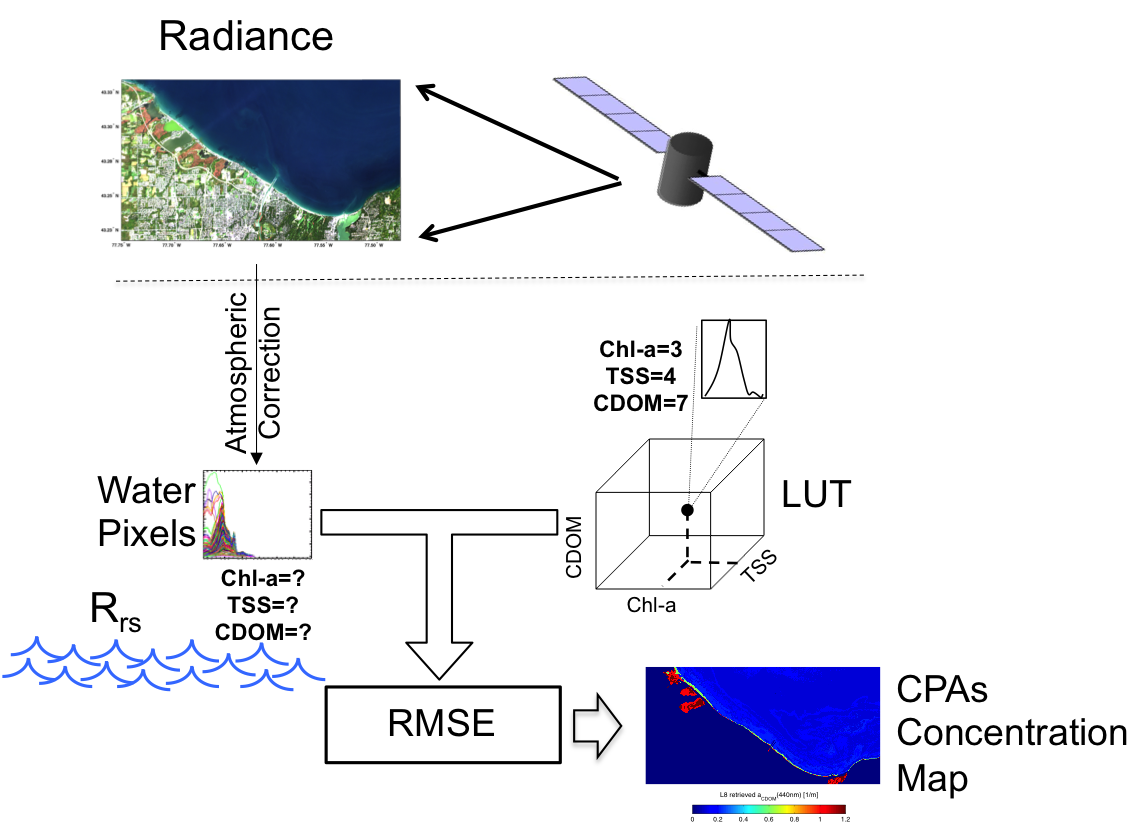
\includegraphics[height=15cm]{./Images/Retrieval_RMSE.png}
    \caption{Retrieval process flow diagram.   \label{fig:retrieval} }
\end{figure}
\end{center}
\end{block}



\end{column}   

%%%%%%%%%%%%%%%%%%%%%%%%%%%%%%%%%%%%%%%%%%%%%%%%%%
% COLUMN 2      %%%%%%%%%%%%%%%%%%%%%%%%%%%%%%%%%%%%%%%%
 \begin{column}{.31\linewidth}  %.29\linewidth (3-columns) %0.46\linewidth (2-columns)
%%%%%%%%%%%%%%%%%%%%%
% BLOCK 1 (column 2) 
%%%%%%%%%%%%%%%%%%%%%
%-------------------------------

% -----------------------------------------------
\begin{block}{Hydrolight}
\small
\begin{itemize}
  \item In-water radiative transfer model
  \vspace{0.5cm}
  \item Inputs: inherent optical properties (IOPs), IOPs concentrations, geometry, etc.
  \vspace{0.5cm}
  \item Output: spectral $R_{rs}$, radiance distributions and derived quantities (irradiances, K functions, etc.)
  \vspace{0.5cm}
  \item Used for the Dark Pixel reflectance determination and for the LUT generation
\end{itemize}
\vspace{1cm}
\begin{figure}[H]
    \includegraphics[height=18cm]{/Users/javier/Desktop/Javier/PHD_RIT/ConferencesAndApplications/2014_ASPRS_SOY/Images/HLdiagram.pdf}
    \caption{Hydrolight model}
\end{figure}
% \hspace{12cm}{\scriptsize $*~$IOPs: Inherent Optical Properties}
% \vspace{1cm}
\end{block}

% -----------------------------------------------

\begin{block}{AC: Model-Based ELM (MoB-ELM)}

% ----------------------------------------------
\begin{itemize}
  \item \small Empirical Line Method (ELM): Linear relationship between radiance $L$ and reflectance $r_d$:
\begin{equation}\label{eq:ELM}
  L(\lambda)=m\times r_d(\lambda)+b
\end{equation}

\vspace{0.005cm}
\item \small At least two pixels from the scene: {\bf \small Dark} and {\bf \small Bright} Pixels with known reflectances

\end{itemize}

\begin{figure}[htb]
  \centering
\resizebox{14cm}{!}{%
\begin{tikzpicture}[x=2.8ex,y=.7ex]
  %axis
  \draw (0,0) -- coordinate (x axis mid) (10,0);
    \draw (0,0) -- coordinate (y axis mid) (0,30);
    %labels      
  \node[below=0ex] at (8,0) {\small $Band_i~~reflectance~(r_d)$};
  \node[rotate=90] at (-.5,23) {\small $Band_i~~Radiance~(L)$};

  \node[below=.2ex] at (-2.1,4.5) {\small $b=$offset};
  \node[below=1.4ex] at (-2.1,4.0) {\scriptsize (path radiance)};
  \draw[rotate=90,|<->|] (0,1) -- coordinate (x axis mid) (1,1);

  \node[below=0ex] at (2,16) {\small Dark Object};
  \draw[arrows=-triangle 45] (2,12.5) -- (2,9);

  \node[below=0ex] at (4,21) {\small $m=$ Slope};
  \draw[arrows=-triangle 45] (4,17.5) -- (5,14.5);

  \node[below=0ex] at (7,28) {\small Bright Object};
  \draw[arrows=-triangle 45] (7,24.5) -- (7.9,20.5);

  \node[below=0ex] at (8,9) {\small $r_d=(L-b)/m$};

  %plots
  \draw plot 
    file {linereg.data};
  \draw plot[mark=*] 
    file {linereg2.data};

\end{tikzpicture}
  }%close \resizebox
\caption{Regression used in MoB-ELM \label{fig:ELM}}
\end{figure}

\vspace{1cm}

{\large \bf Bright Pixel}
\vspace{0.5cm}
\begin{itemize}
    \item Radiance: pseudo-invariant features (PIF) from Landsat 8 image
    \vspace{0.5cm}
    \item Reflectance: PIF from Landsat reflectance product
\end{itemize}
\vspace{1.0cm}
{\large \bf Dark Pixel}
\vspace{0.5cm}
\begin{itemize}
    \item Radiance: region of interest (ROI) over water from Landsat 8 image
    \vspace{0.5cm}
    \item Reflectance: Hydrolight with known IOPs from the ROI
\end{itemize}
\vspace{0.5cm}



\begin{figure}[htb]
  \begin{minipage}[c]{0.49\linewidth}
    \centering
      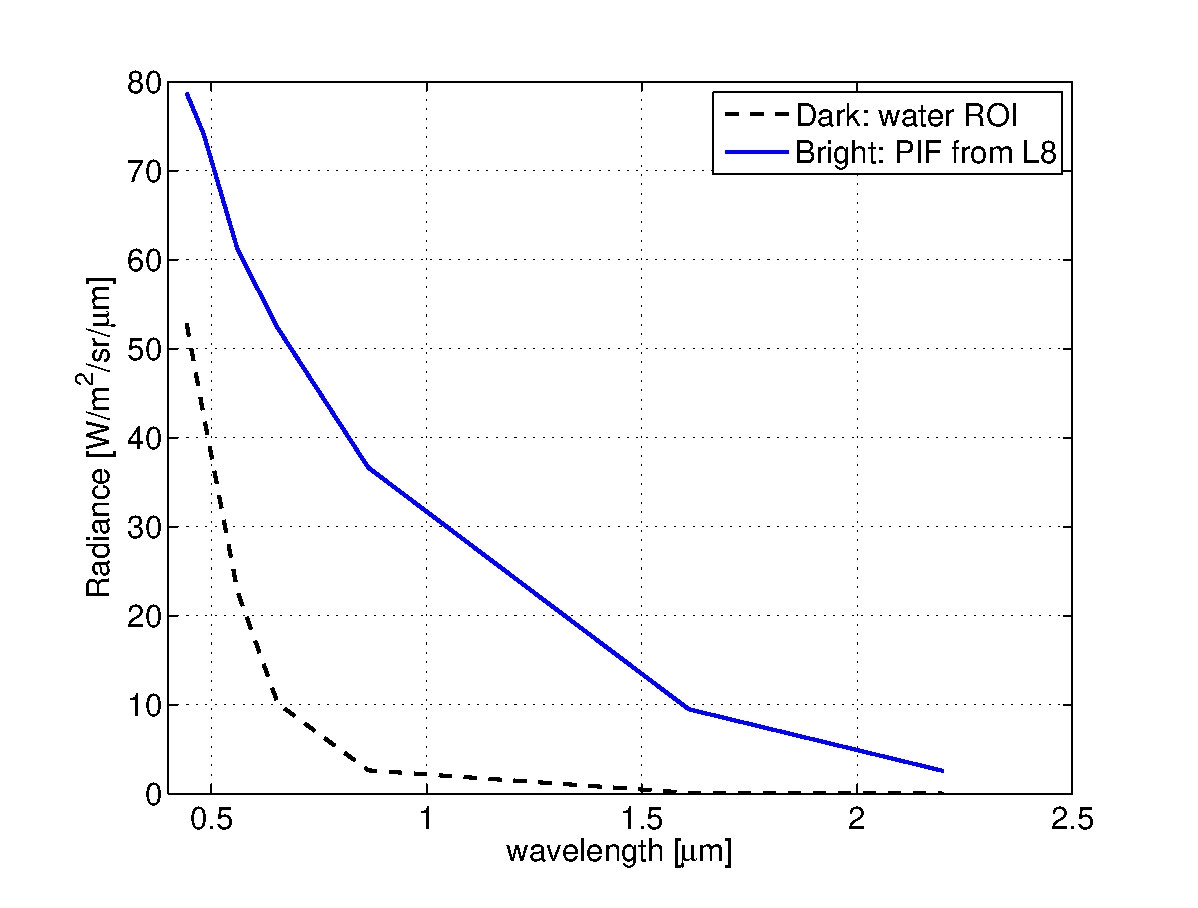
\includegraphics[width=13cm]{/Users/javier/Desktop/Javier/PHD_RIT/ConferencesAndApplications/2015_Landsat_Special_Issue/Images/ELMrad130929_150422}\\
    % \vspace{1.5cm}
    \centerline{\small (a)}\medskip
  \end{minipage}
  \begin{minipage}[d]{0.49\linewidth}
    \centering
      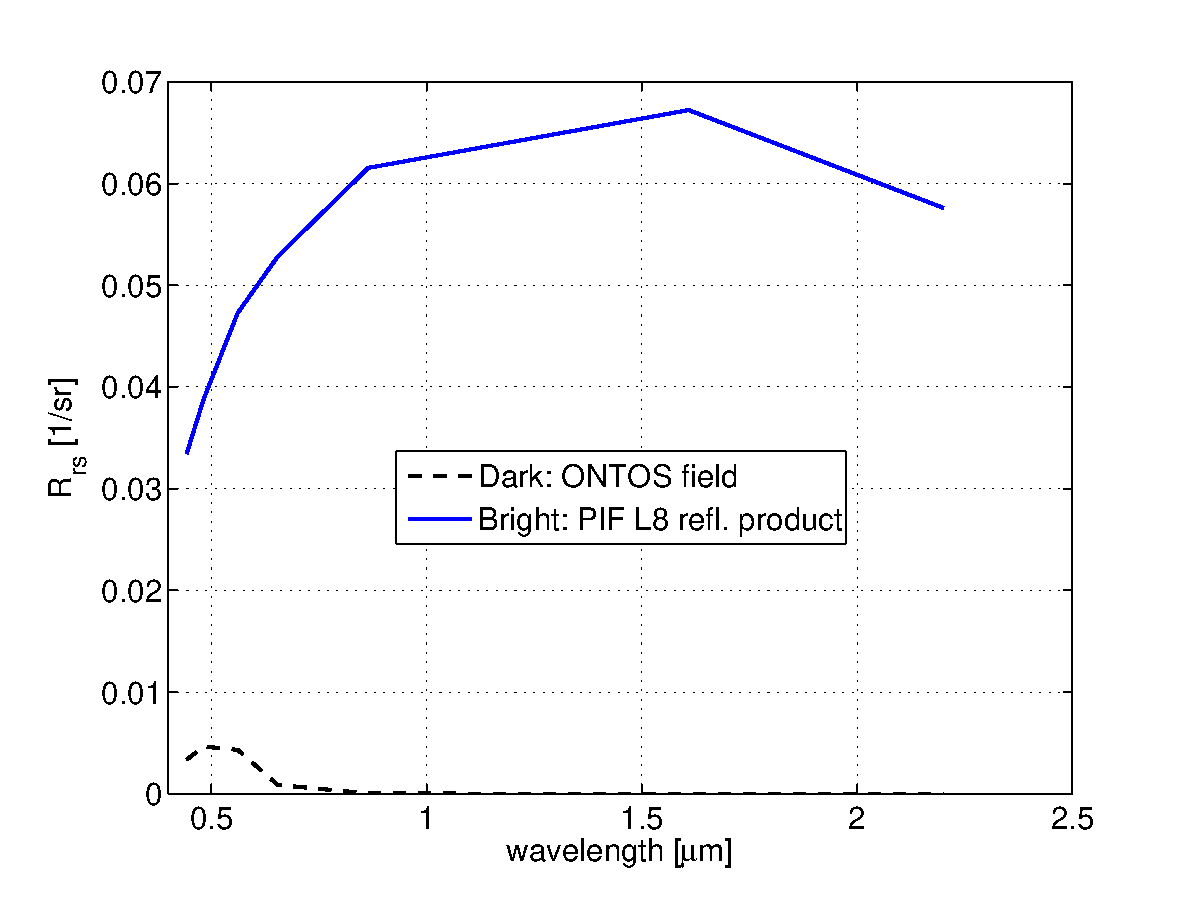
\includegraphics[width=13cm]{/Users/javier/Desktop/Javier/PHD_RIT/ConferencesAndApplications/2015_Landsat_Special_Issue/Images/ELMRrs130929_150422}\\
    % \vspace{1.5cm}
    \centerline{\small (b)}\medskip
  \end{minipage}
  \caption{Example of the (a) radiance and (b) $R_{rs}$ for the bright and dark pixel used in the MoB-ELM for Landsat 8 scene acquired on 09-19-2013.\label{fig:MOBELMpxls} } 
\end{figure}

\begin{figure}[htbp!]
  \centering
  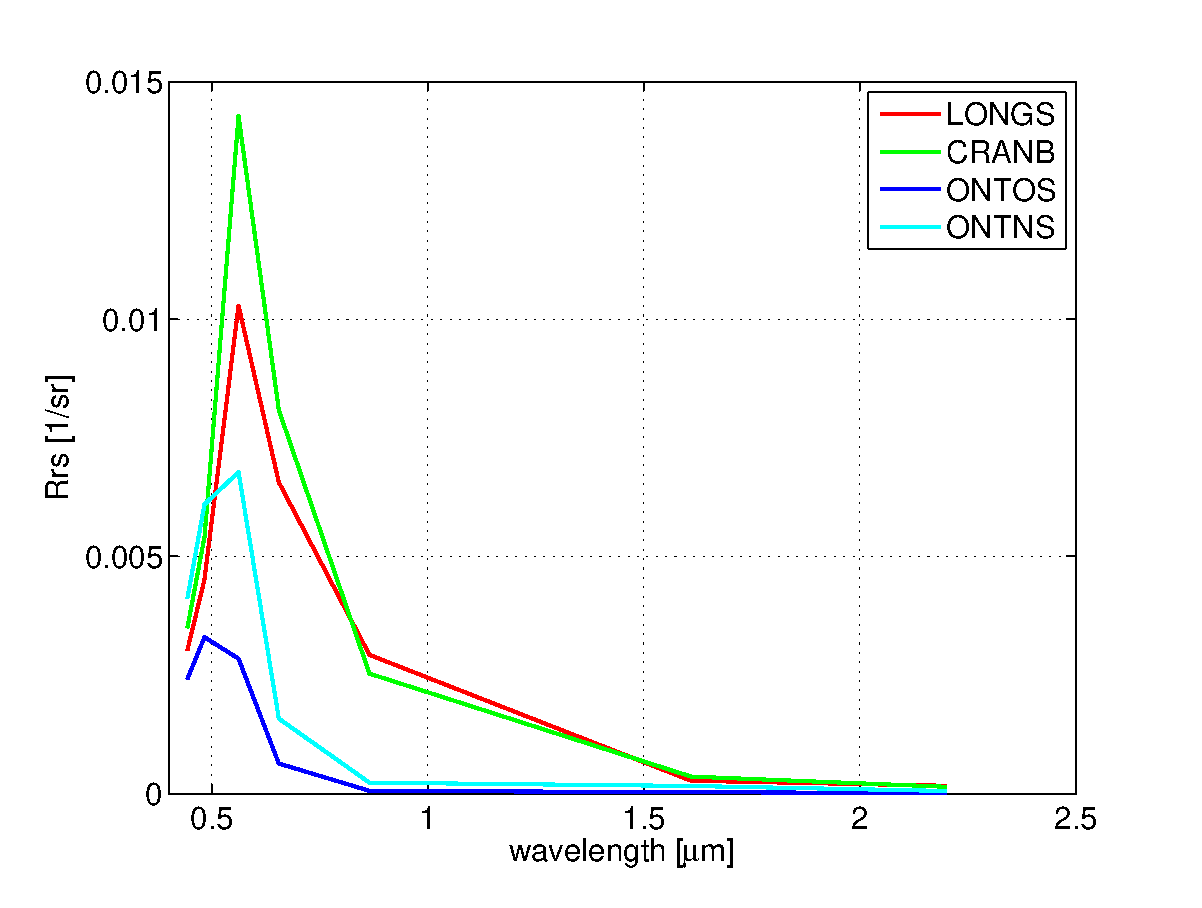
\includegraphics[width=14cm]{/Users/javier/Desktop/Javier/PHD_RIT/ConferencesAndApplications/2015_Landsat_Special_Issue/Images/ROI130919_150422}
  \caption{$R_{rs}$ for the sites for the 09-19-2013 collection after applying the MoB-ELM atmospheric correction.\label{fig:RrsROIs130919} } 
\end{figure}
\vspace{-.2cm}
\end{block}


\end{column}
%%%%%%%%%%%%%%%%%%%%%%%%%%%%%%%%%%%%%%%%%%%%%%%%%
%COLUMN 3
%%%%%%%%%%%%%%%%%%%%%%%%%%%%%%%%%%%%%%%%%%%%%%%%%
 \begin{column}{.31\linewidth}
%%%%%%%%%%%%%%%%%%%%%        
% Block 1 (column 3)      
%%%%%%%%%%%%%%%%%%%%%
% \vspace{.5cm}
%-----------------------
\begin{block}{Look-Up Table}


\begin{table}[htb]
\caption{Input parameters for the LUT generation in Ecolight for the Landsat 8 image acquired on 09-19-2013. \label{tab:LUTconc2}} 
\scriptsize
\centering
    \begin{tabular}{c|c|c|c|c}
    \hline \hline
            IOPs Input & \bfseries{$C_a$} & \bfseries{$TSS$} & \bfseries{$a_{CDOM}(440nm)$} & \bfseries{$b_b/b$}    \\
                   & $[mg~m^{-3}]$        & $[g~m^{-3}]$       &  $[1/m]$           & $[\%]$            \\ \hline \hline
ONTNS   &  0.1    & 1.0     &  0.11   &  0.3  \\
--    &  0.5    & 2.0     &  0.15   &  0.4  \\
--      &  1.0    & 5.0     &  0.21   &  0.5  \\
--      &  3.0    & 10.0    &  0.6    &  0.6  \\ 
--    &  10.0     & --    &  --   &  0.7  \\  
--      &  20.0     & --    &  --   &  1.0  \\  
--      &  40.0     & --    &  --   &  1.4  \\
--      &  --       & --    &  --   &  2.0  \\ \hline

LONGS   &  60.0   & 25.0    &  1.0    &  0.3  \\
--      &  90.0   & 45.0    &  1.2    &  0.4  \\
--      &  110.0  & 50.0    &  --     &  0.5  \\
--      &  --     & --      &  --     &  0.6  \\  
--      &  --     & --      &  --     &  0.7  \\  
--      &  --     & --      &  --     &  1.0  \\   
--      &  --     & --      &  --     &  1.4  \\  
--      &  --     & --      &  --     &  2.0  \\  \hline \hline
% --      &  135.0  & --      &  --     &  --   \\  
% --      &  150.0  & --      &  --     &  --   \\ \hline 
    \end{tabular}
  \end{table}


\begin{figure}[htb]
    \centering
      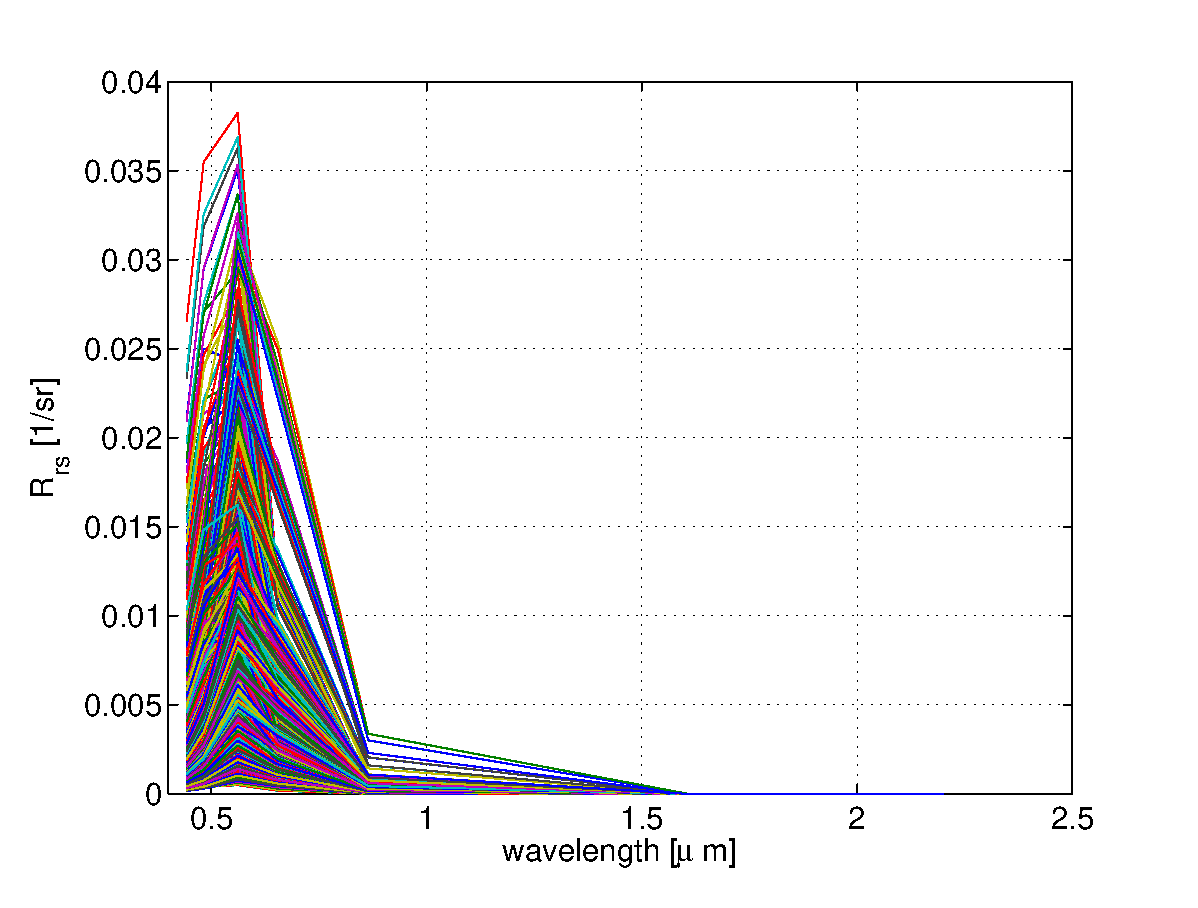
\includegraphics[width=14cm]{/Users/javier/Desktop/Javier/PHD_RIT/ConferencesAndApplications/2015_Landsat_Special_Issue/Images/LUTsmart130919_150422.eps}
      \caption{LUT with $1170$ elements created in Ecolight for the Landsat 8 scene acquired on 09-19-2013. Each element was created from a combination of parameters in Table \autoref{tab:LUTconc2}.}
      \label{fig:LUT}

\end{figure}


\end{block}
%-------------------------------------
\begin{block}{Retrieval}
  \begin{itemize}
    \item Spectral matching technique to predict concentration of CPAs
    \vspace{0.5cm}
    \item Comparison between spectral shape of water pixel (unknown concentrations) with the LUT (known concentrations) in the least-squared sense using the RMSE
  \end{itemize}
\end{block}

\begin{block}{Results}

\begin{figure}[htbp!]
  \begin{minipage}[c]{0.46\linewidth}
      \centering
      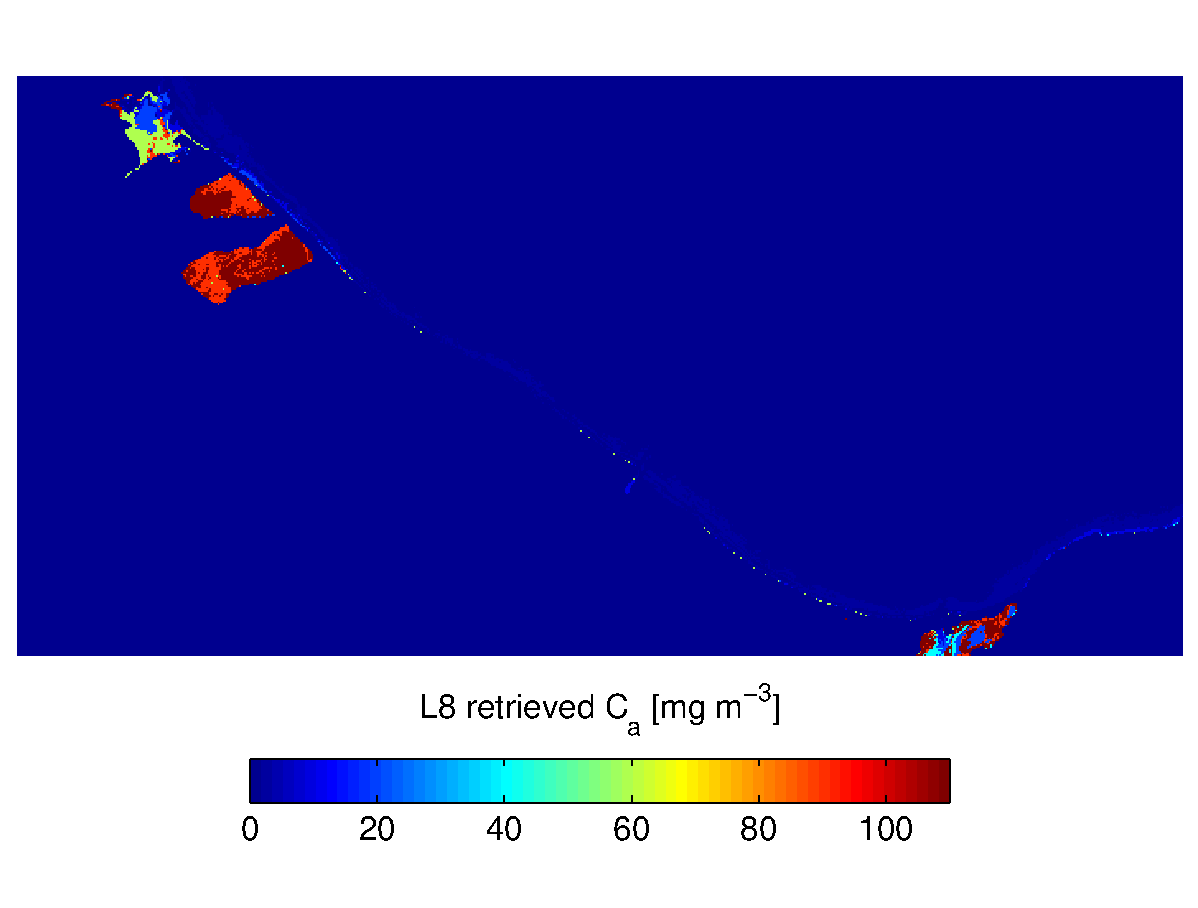
\includegraphics[trim=0 20 0 30,clip,height=8.0cm]{/Users/javier/Desktop/Javier/PHD_RIT/ConferencesAndApplications/2015_Landsat_Special_Issue/Images/CHLmap130919_150420}  
  \end{minipage}
  \hspace{1cm}
  \begin{minipage}[c]{0.46\linewidth}
      \centering
      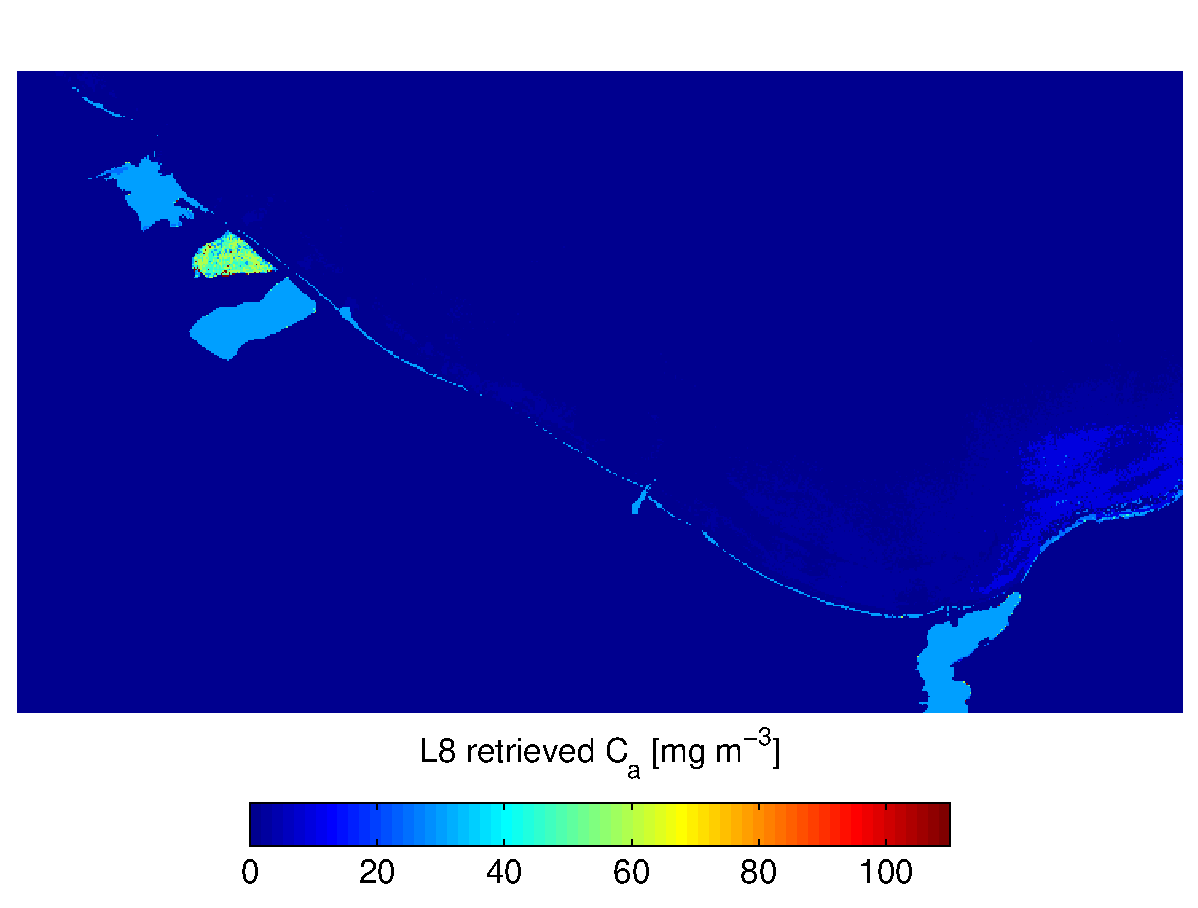
\includegraphics[trim=0 0 0 30,clip,height=8.0cm]{/Users/javier/Desktop/Javier/PHD_RIT/ConferencesAndApplications/2015_Landsat_Special_Issue/Images/CHLmap140929_150420}  
  \end{minipage}
% 
%% TSS
  \begin{minipage}[c]{0.46\linewidth}
      \centering
      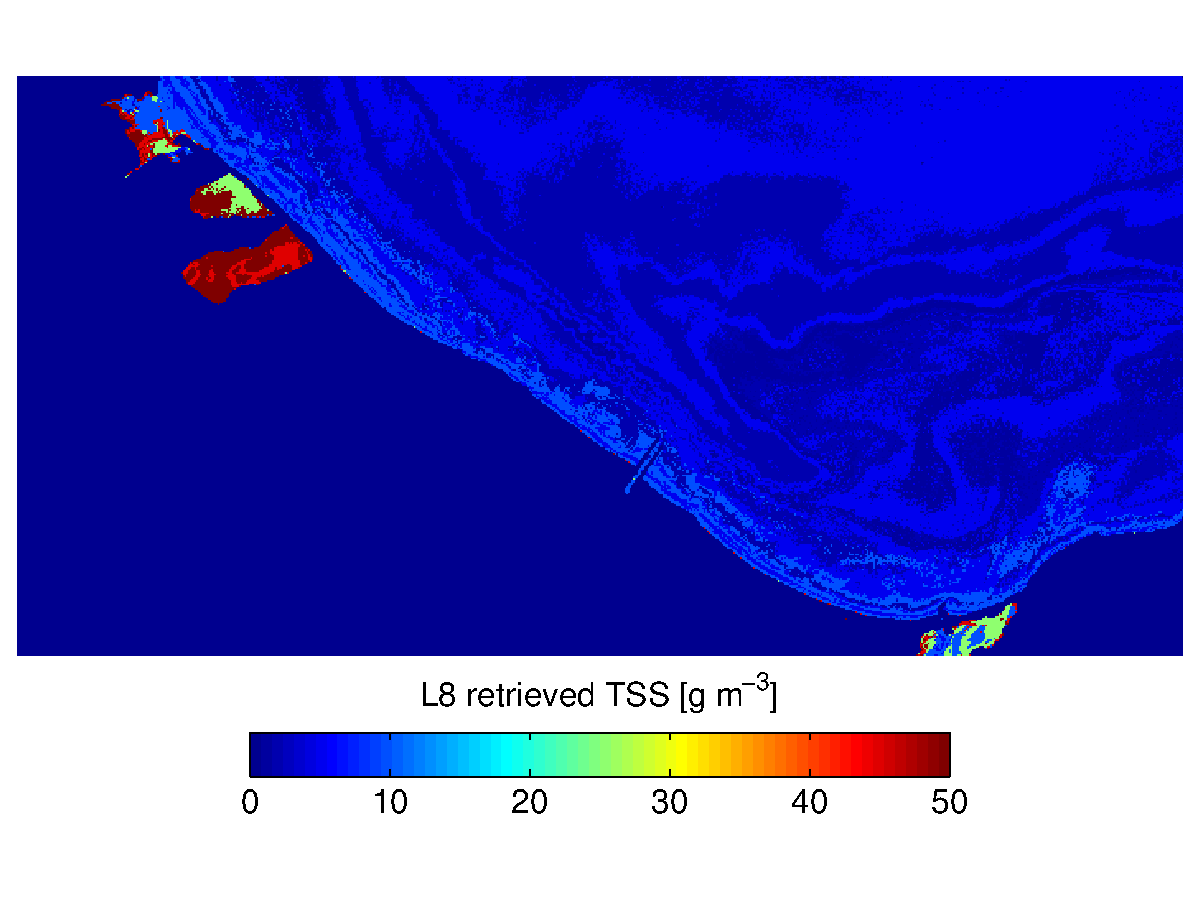
\includegraphics[trim=0 30 0 10,clip,height=8.0cm]{/Users/javier/Desktop/Javier/PHD_RIT/ConferencesAndApplications/2015_Landsat_Special_Issue/Images/TSSmap130919_150420}  
  \end{minipage}
  \hspace{1cm}
  \begin{minipage}[c]{0.46\linewidth}
      \centering
      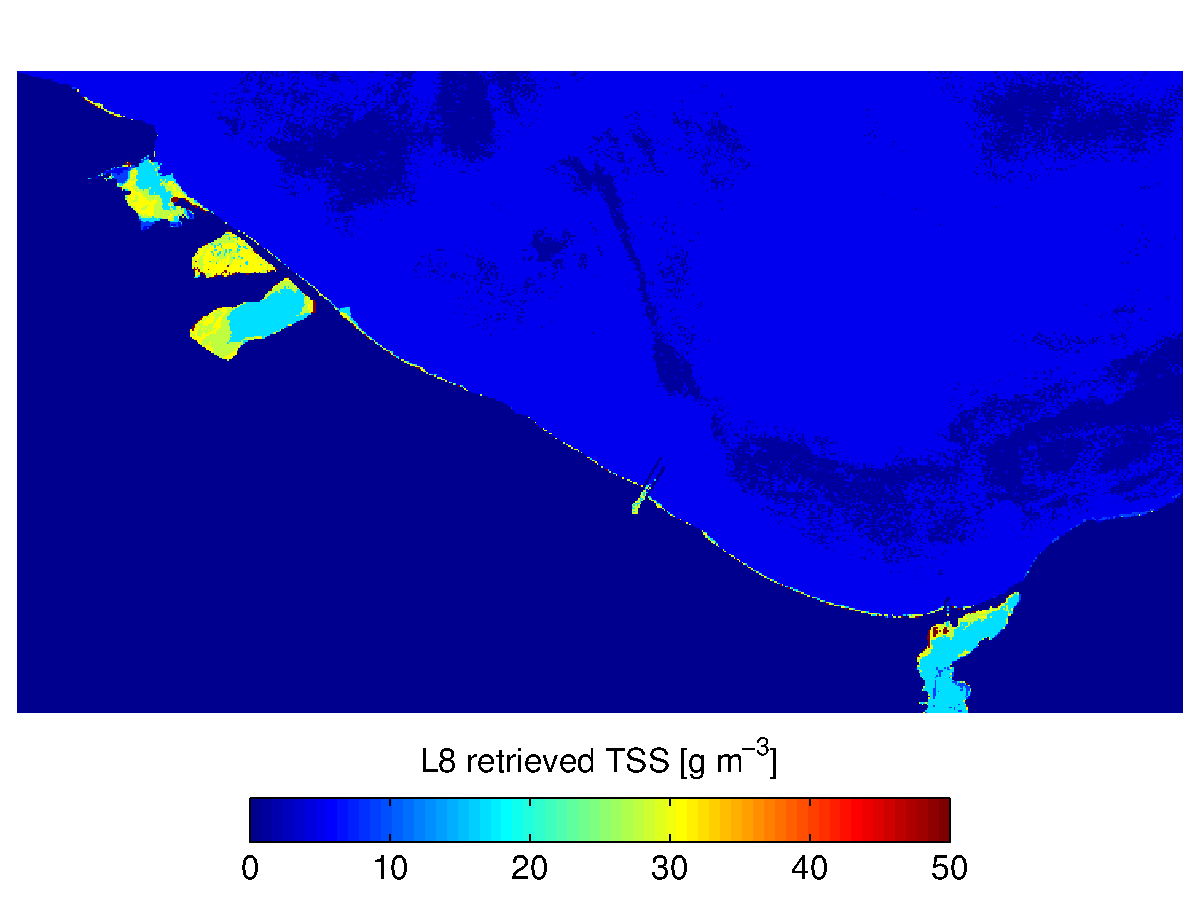
\includegraphics[trim=0 0 0 30,clip,height=8.0cm]{/Users/javier/Desktop/Javier/PHD_RIT/ConferencesAndApplications/2015_Landsat_Special_Issue/Images/TSSmap140929_150420}  
  \end{minipage}

%% CDOM
  \begin{minipage}[c]{0.46\linewidth}
      \centering
      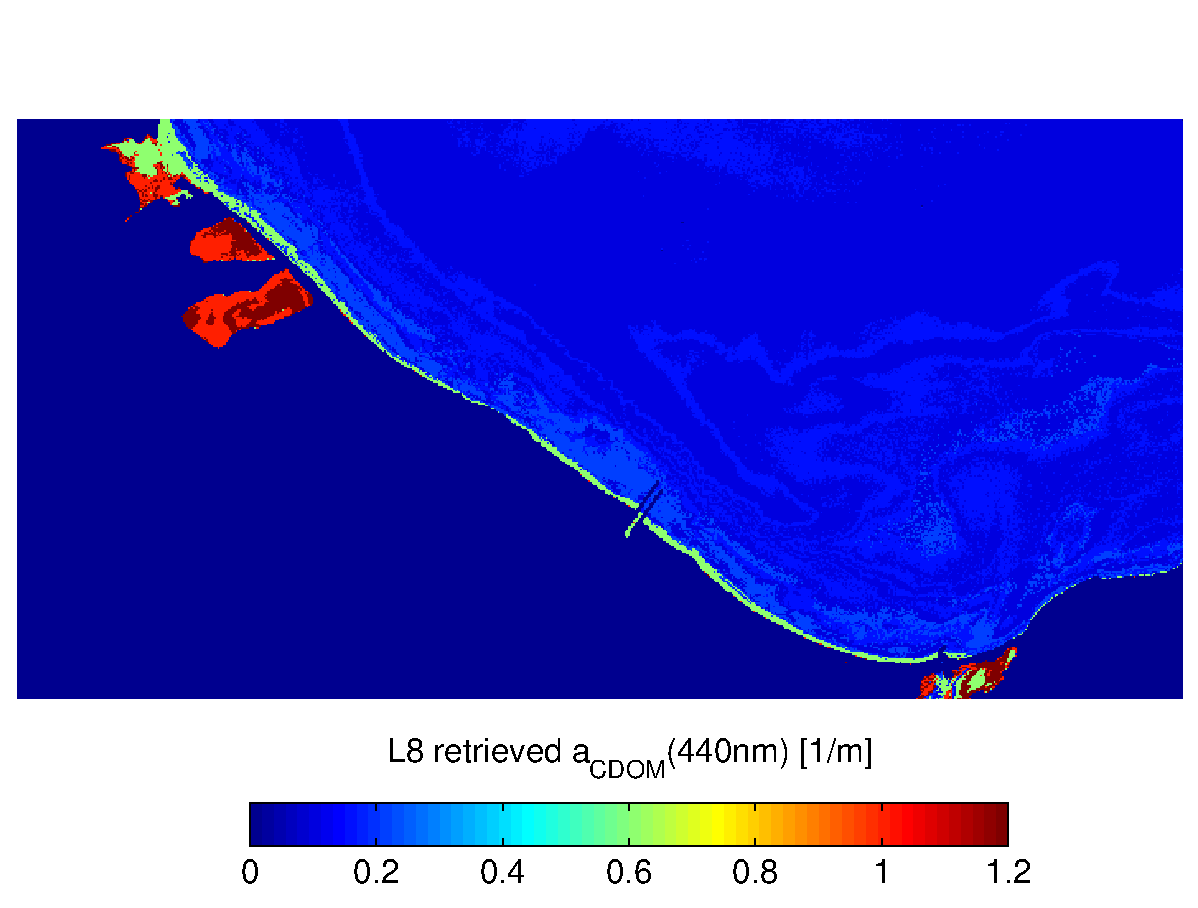
\includegraphics[trim=0 0 0 30,clip,height=8.0cm]{/Users/javier/Desktop/Javier/PHD_RIT/ConferencesAndApplications/2015_Landsat_Special_Issue/Images/CDOMmap130919_150420}\\
      \centerline{\small (a)}  
  \end{minipage}
  \hspace{1cm}
  \begin{minipage}[c]{0.46\linewidth}
      \centering
      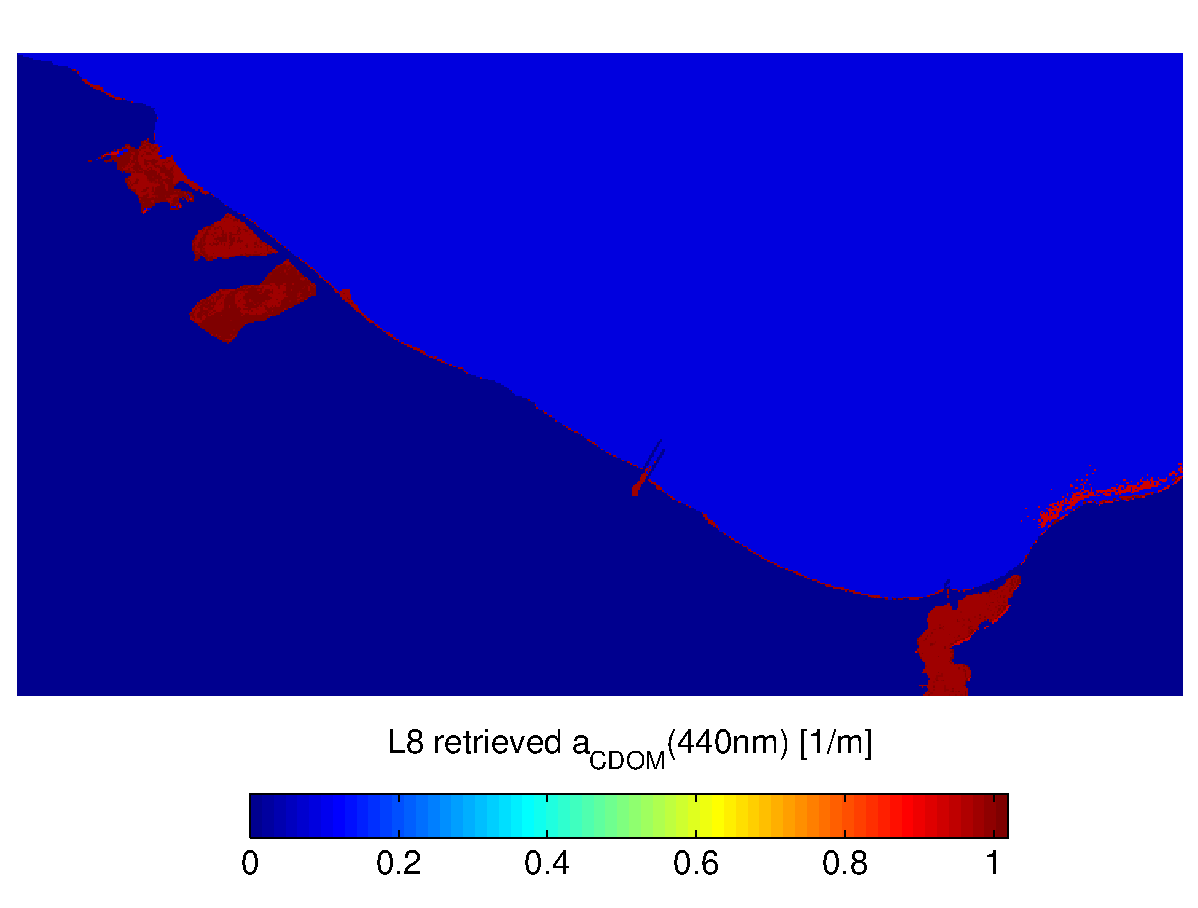
\includegraphics[trim=0 0 0 30,clip,height=8.0cm]{/Users/javier/Desktop/Javier/PHD_RIT/ConferencesAndApplications/2015_Landsat_Special_Issue/Images/CDOMmap140929_150420}\\
      \centerline{\small (b)}
  \end{minipage}
  \caption{CPA concentration retrieval results for the Landsat 8 images acquired on (a) 09-19-2013 and (b) 09-29-2014.} 
\end{figure}


\begin{figure}[htb]
  \begin{minipage}[c]{0.47\linewidth}
      \centering
  % CHL
      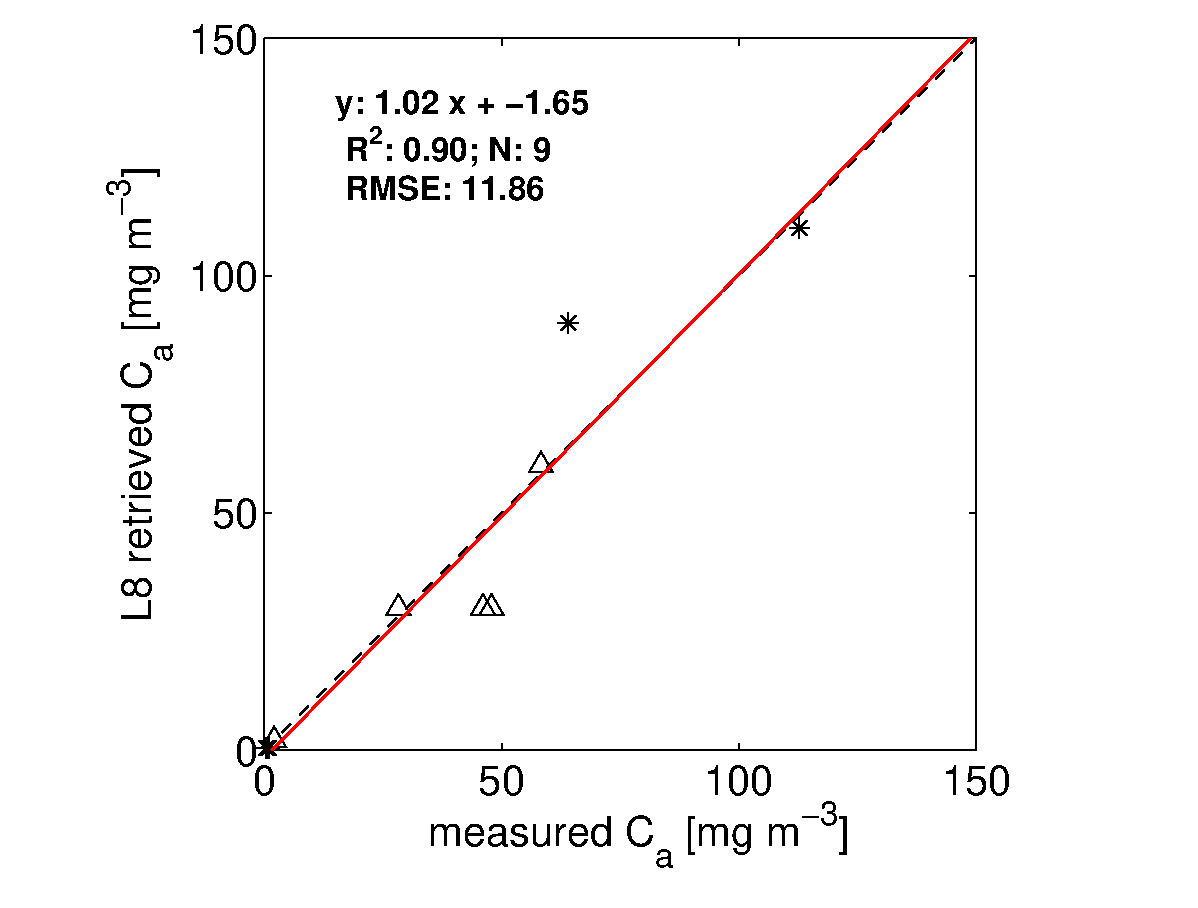
\includegraphics[trim=40 0 80 0,clip,height=9.0cm]{/Users/javier/Desktop/Javier/PHD_RIT/ConferencesAndApplications/2015_Landsat_Special_Issue/Images/CHLretvsmea150423} 
  \end{minipage}
  \hspace{0.5cm}
  % TSS
  \begin{minipage}[d]{0.47\linewidth}
      \centering
      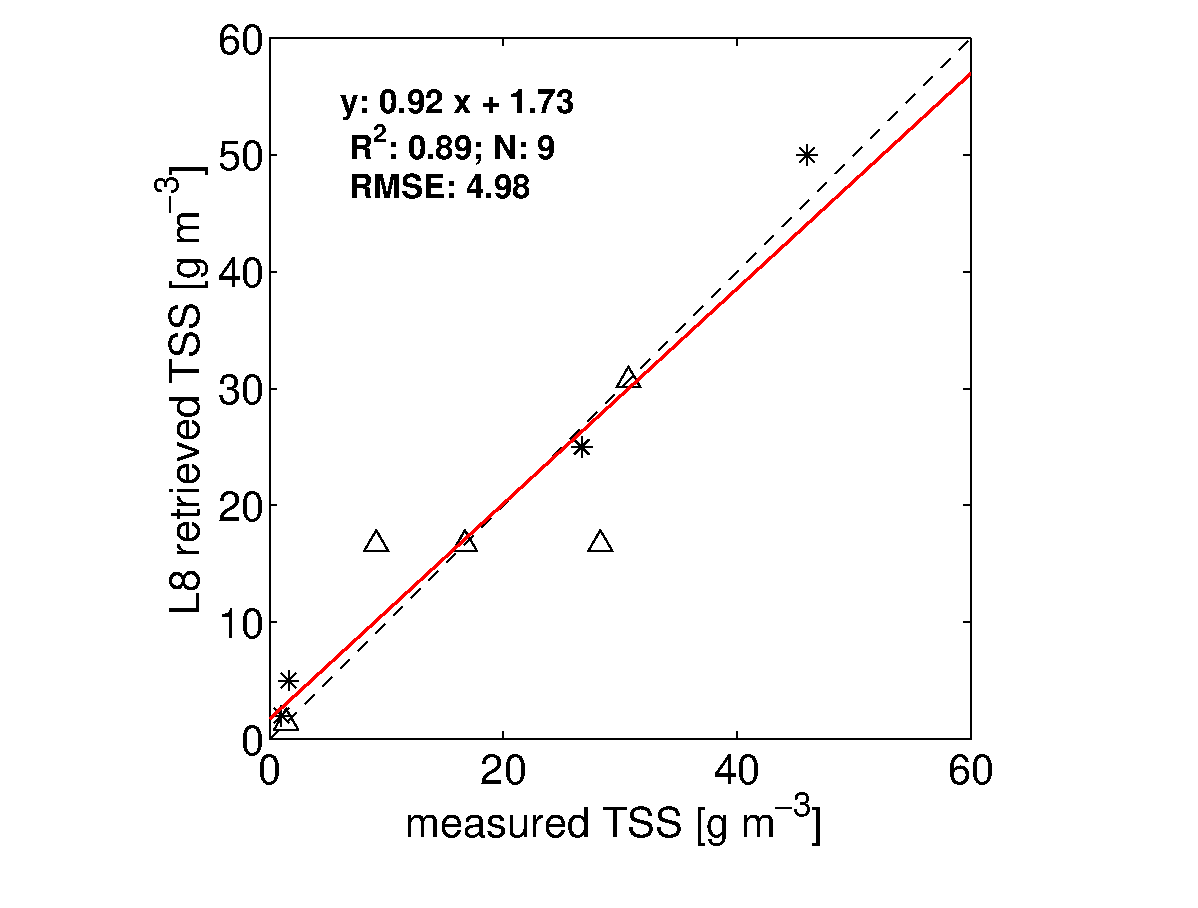
\includegraphics[trim=40 0 80 0,clip,height=9.0cm]{/Users/javier/Desktop/Javier/PHD_RIT/ConferencesAndApplications/2015_Landsat_Special_Issue/Images/TSSretvsmea150423}
  \end{minipage}\\
  % CDOM
  \begin{minipage}[c]{0.47\linewidth}
      \centering
      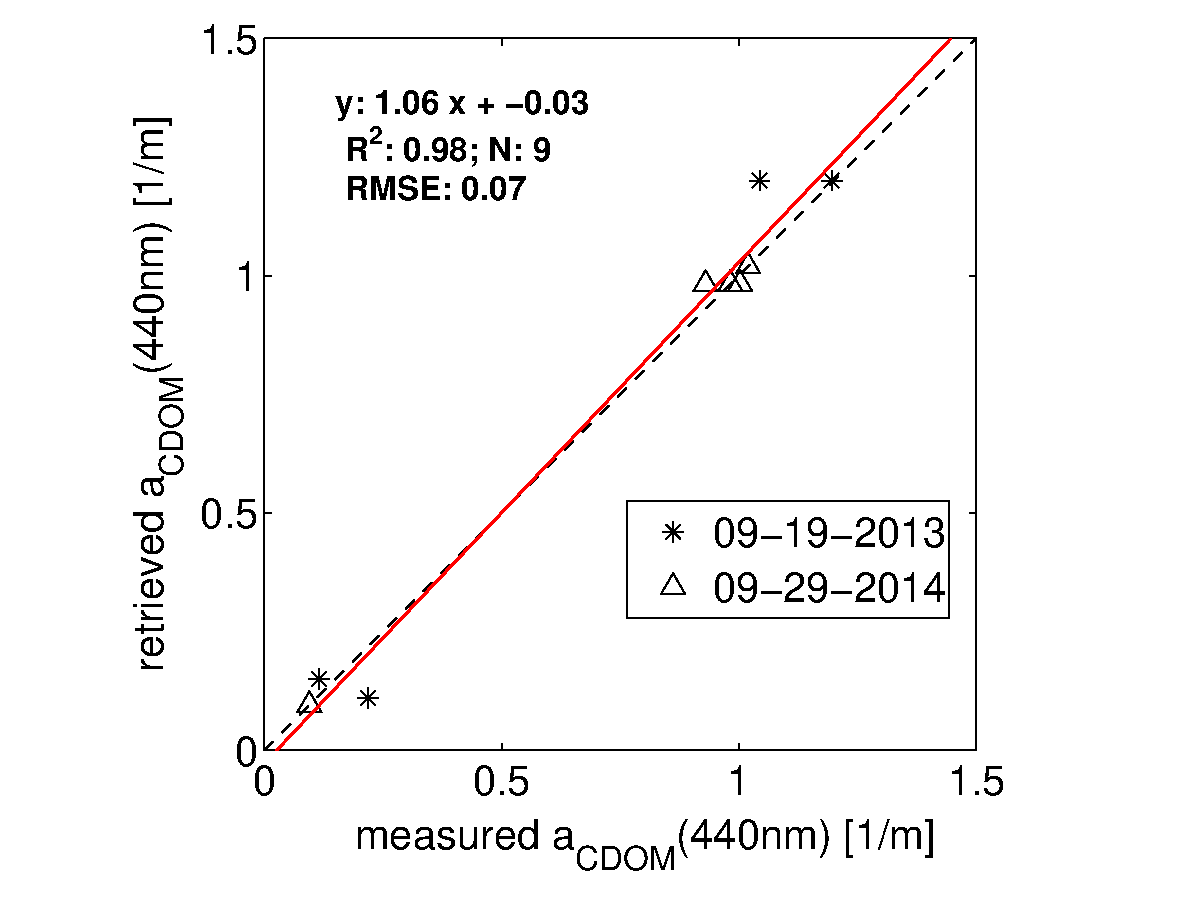
\includegraphics[trim=40 0 80 0,clip,height=9.0cm]{/Users/javier/Desktop/Javier/PHD_RIT/ConferencesAndApplications/2015_Landsat_Special_Issue/Images/CDOMretvsmea150423}  
  \end{minipage}
  \hspace{0.5cm}
  \begin{minipage}[c]{0.47\linewidth}
      \centering
      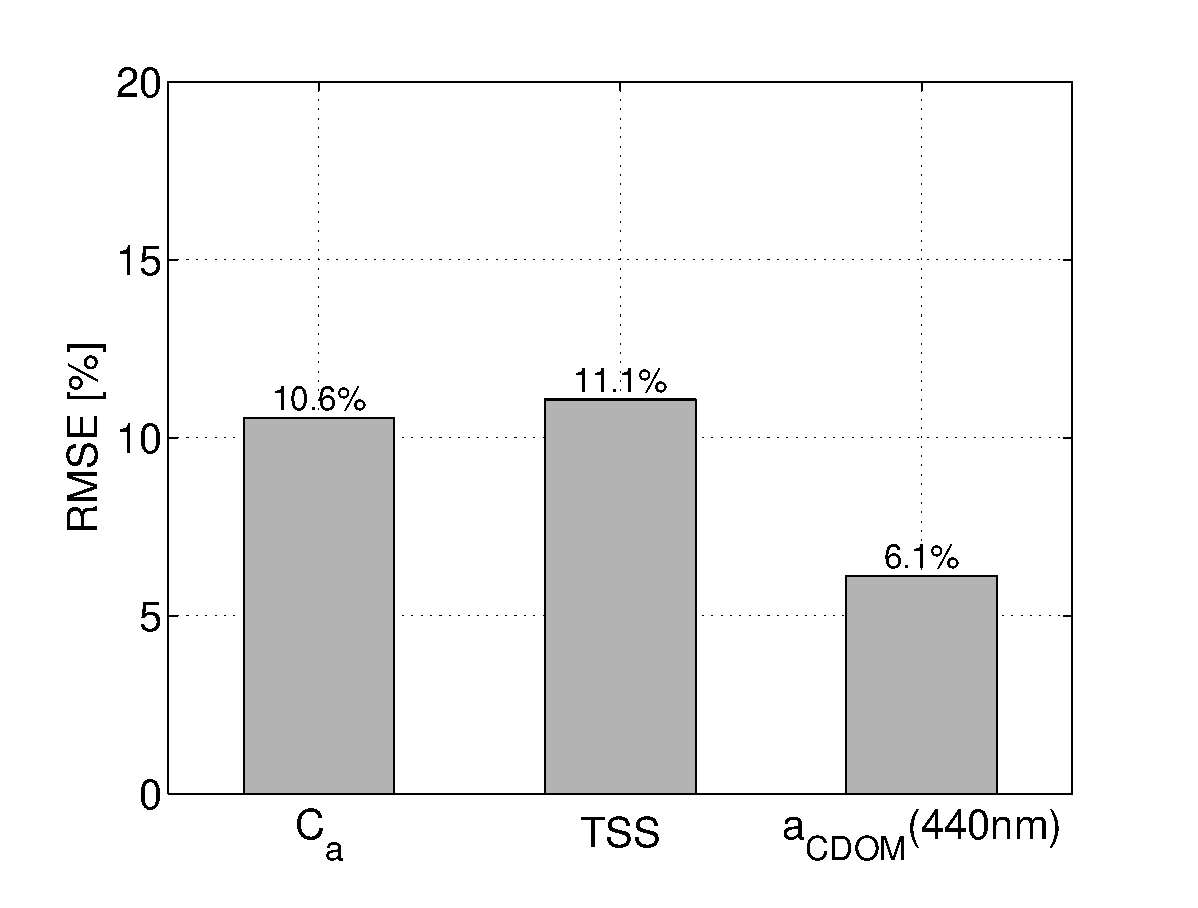
\includegraphics[height=9.0cm]{/Users/javier/Desktop/Javier/PHD_RIT/ConferencesAndApplications/2015_Landsat_Special_Issue/Images/RMSE_ret150421}
  \end{minipage}

  \caption{Landsat 8's retrieved vs measured CPA concentration for the 09-19-2014 and 09-29-2015 scenes with regression line (solid red line) and goodness of fit values and RMSE expressed as percentage of range for each CPA (lower right). The dashed line represents the 1:1 line. \label{fig:CPAsRetVSMea} } 
\end{figure}        

  %-------------   

\end{block}  
%%%%%%%%%%%%%%%%%%%%%%%%%%%%%%%%%%%%%%%%%%%%%%%%%


% \begin{block}{Conclusion}
	
% \justifying\small A retrieval process to simultaneously retrieve the CPAs using Landsat 8 images was developed. The first step is to atmospherically correct the image using a model-based ELM that uses PIF extraction for the bright pixel determination and the radiative transfer model Hydrolight for the dark pixel. Then, an nonlinear optimization routine is used to estimate the CPAs concentration for each water pixel from the LUT created in Hydrolight. Initial results were presented that exhibit expected trend for the concentration in the lake and nearby ponds. A comparison with field measurements showed good agreement at low concentrations but differences at higher concentrations.
% \vspace{.3cm}
% \end{block}


% \begin{block}{References} 
   
%  { \scriptsize 
% \setbeamertemplate{bibliography item}[text]
% 				\bibliographystyle{spiebib}
% 				\bibliography{/Users/javier/Desktop/Javier/PHD_RIT/Latex/javier_bib}
% }
% \end{block} 

\end{column}
 %%%%%%%%%%%%%%%%%%%%%%%%%%%%%%%%%%%%%%%%%%%%%%%%%%%%%%%%%%%%%%%%%%%%%%%%%%%%%%%%%%
\end{columns}
\end{frame}

\end{document}


%%%%%%%%%%%%%%%%%%%%%%%%%%%%%%%%%%%%%%%%%%%%%%%%%%%%%%%%%%%%%%%%%%%%%%%%%%%%%%%%%%%%%%%%%%%%%%%%%%%%
%%% Local Variables: 
%%% mode: latex
%%% TeX-PDF-mode: t
%%% End:

%spelling checked
